
\section{Application Evaluation}
\label{sec:apps}
Legion\cite{Legion12} is a high-level runtime system that has been implemented on top
of our interface.  
%The Legion runtime is distributed so 
%that there is an independent scheduler for each processor in the machine.  
The Legion programming model is built around the abstraction of 
{\em logical regions} which express locality and independence properties 
of data.  Computation in Legion is organized into a tree of tasks where 
each task must specify which logical regions will be accessed.
When executing a Legion task, the Legion runtime receives requests
to execute sub-tasks along with their region requirements.
This stream of tasks with region requirements is analogous to a stream
of instructions with register requirements that are executed by 
a hardware processor.  Hardware out-of-order processors are designed to
run ahead of the actual execution of a stream of instructions
to ensure that the processor's pipeline is fully utilized.  Similarly, in a
Legion application, for every processor there is an instance of the Legion runtime
that takes a stream of tasks with region requirements and asynchronously
runs ahead of the actual execution using a scheduler called a {\em Software Out-of-Order Processor} 
(SOOP).  The SOOP leverages our interface by asynchronously issuing task launches, copy
operations, and synchronization operations with the dependencies between them expressed
as events.  The full details of the SOOP are beyond the scope of this paper
and are described in \cite{Legion12}.

The fully asynchronous design of the interface proposed in
this paper is crucial to Legion's SOOP implementation.  Without a fully
asynchronous interface, the SOOP would have to periodically invoke
blocking operations that would cause processors to stall and severely
limit Legion's ability to run ahead and keep the machine fully
occupied.  With a fully asynchronous interface the SOOP can hide latencies by 
running
far ahead of the actual execution, limited only by the physical resources
available in the machine, exactly like a hardware out-of-order processor.

In this section we demonstrate the performance properties of three
real-world applications that use the Legion runtime and the heterogeneous
implementation of our interface to run on the Keeneland supercomputer.
The three applications that we characterize are all multi-phase
applications that require parallel computation, data exchange, and
synchronization between phases. 

{\em Circuit} is a simulation of an integrated circuit that is described as an
irregular graph of components connected by wires.  The graph is partitioned
and distributed across the machine.  The computation for each time step consists
of three phases that calculate currents on the wires, distribute charge between
components, and update the voltages of all components.  In the distribute charge
phase, a single component may be updated by wires from multiple partitions.  Reduction instances 
are used to allow each partition to perform reductions in parallel and to do so locally in GPU
framebuffer memory before merging all the reductions to a global instance
residing in GASNet memory.  Without reduction instances this phase
couldn't be performed using GPUs.

{\em Fluid} is an incompressible fluid flow simulation from the PARSEC
benchmark suite\cite{bienia11benchmarking}.  The reference implementation can 
only be run on a single shared memory machine, but when written in Legion, Fluid can
be run on large distributed machines as well.  The Fluid simulation
models particles that flow through cells.  Each time step requires multiple phases
that update different properties of the particles contingent upon neighboring
particles in the same cell.  The space of cells is partitioned and neighboring
cells in different partitions must exchange data between phases.  Legion ensures
that these exchanges are done point-to-point by chaining copies and tasks
using events rather than employing a global bulk-synchronous approach.

{\em AMR} is an adaptive mesh refinement benchmark based on the third heat
equation example from the Berkeley Labs BoxLib project\cite{BoxLib}.  AMR
simulates the two dimensional heat diffusion equation using three different levels
of refinement.  Each level is partitioned and distributed across the machine.  Time steps require
both intra- and inter-level communication and synchronization.  Legion again
expresses dependences between tasks from the same and different levels through
events.

In Section~\ref{subsec:eventlife} we study the lifetime of events in
the Fluid application.  Section~\ref{subsec:lockmig} examines
the migration of locks in the Circuit and AMR applications.  Finally, we demonstrate
that the asynchronous nature of our interface is essential to the
performance of Legion by comparing to bulk-synchronous
implementations of these applications in Section~\ref{subsec:bulkcomp}.
  
\subsection{Event Lifetimes}
\label{subsec:eventlife}

We instrumented the heterogeneous implementation of our interface to 
capture event usage information.  Figure~\ref{fig:eventlife} shows
a timeline of the execution of the Fluid application on 16 nodes.
The dynamic events line measures the total number of event creations.
A large number of events are created - over 260,000 in less than 15
seconds - and allocating separate storage for every event would clearly
be difficult for long-running applications.  

Dynamic events are considered {\em live events} until their last operation 
(i.e. wait, trigger) has been performed.  The live events line
measures the number of events that are live at any given time.  After
the last operation on a dynamic event, a reference counting implementation would
be able to recover the storage associated with the event.  The live events line
is therefore equivalent to the number of needed events in a refernce counting
scheme.  In this example 
a reference counting algorithm would reduce the storage needed for dynamic events
by over 10X, but could only do so at the cost of
computation and communication for performing the reference counting.  

As discussed in Section~\ref{subsec:eventimpl}, our implementation
requires storage that grows with the maximum number of {\em untriggered events}, a number
that is 10X smaller than even the maximal live event count.  The actual storage
requirements of our implementation are shown by the generational events line,
which shows the total number of generational events (defined in Section~\ref{subsec:eventimpl}) 
in the system.
The maximum number of generational events needed is slightly larger than the peak number of untriggered events. 
The reason for this difference is because nodes create events locally if they have
no free generational events, even if there are unused generational events on remote nodes.
Despite this inefficiency, our implementation uses 5X less storage
than a reference counting implementation and avoids any overhead related to 
reference counting.  These savings would likely be even more dramatic for longer 
runs of the application, as the number of live events is steadily growing as the
application runs, while the peak number of generational events needed appears to 
occur during the start-up of the application.

%% much storage would be required for events using 

%%  about different kinds of events.  Figure~\ref{fig:eventlife} shows
%% the lifetimes of different types of events from a single run of the Fluid
%% application on 16 nodes using 8 processors per node.  Dynamic events 
%% is a monotonically increasing line that
%% corresponds to the total number of events created in the system.  By
%% the end of the run, the simulation created over 260,000 dynamic
%% events.  In contrast, the physical events line corresponds to the total number
%% of generational events required to represent the dynamic events 
%% across all the nodes in the system.  Less than 5,000
%% generational events were required to represent all the dynamic events
%% illustrating that the technique of mapping from dynamic events to generational 
%% events described in Section~\ref{subsec:eventimpl} was effective.

%% The live event line shows the total number of {\em live events} at a point in time.  Dynamic events
%% are considered {\em live events} until their last query has been performed.  The number of live
%% events is equivalent to the number of physical events that would be required
%% in a reference counted scheme.  In this case we see that by reusing
%% generational events, we require up to 4X fewer generational events than would be
%% required by a reference counted scheme.

%% In an ideal world the total number of generational events required would be
%% equivalent to the maximum number of generational events in the untriggered
%% state at any point.  The untriggered event line shows the number of generational
%% events in the untriggered state.  We see that the total number of generational
%% events is actually slightly higher than the maximum number of generational
%% events in the untriggered state at any point.  The reason for this is that unused
%% generational events cannot be shared across nodes, so in some cases nodes must
%% make new generational events eventhough there are unused generational events
%% on other nodes.  The small difference in these lines shows that in practice
%% this is only a minor inefficiency.

\begin{figure}
\begin{center}
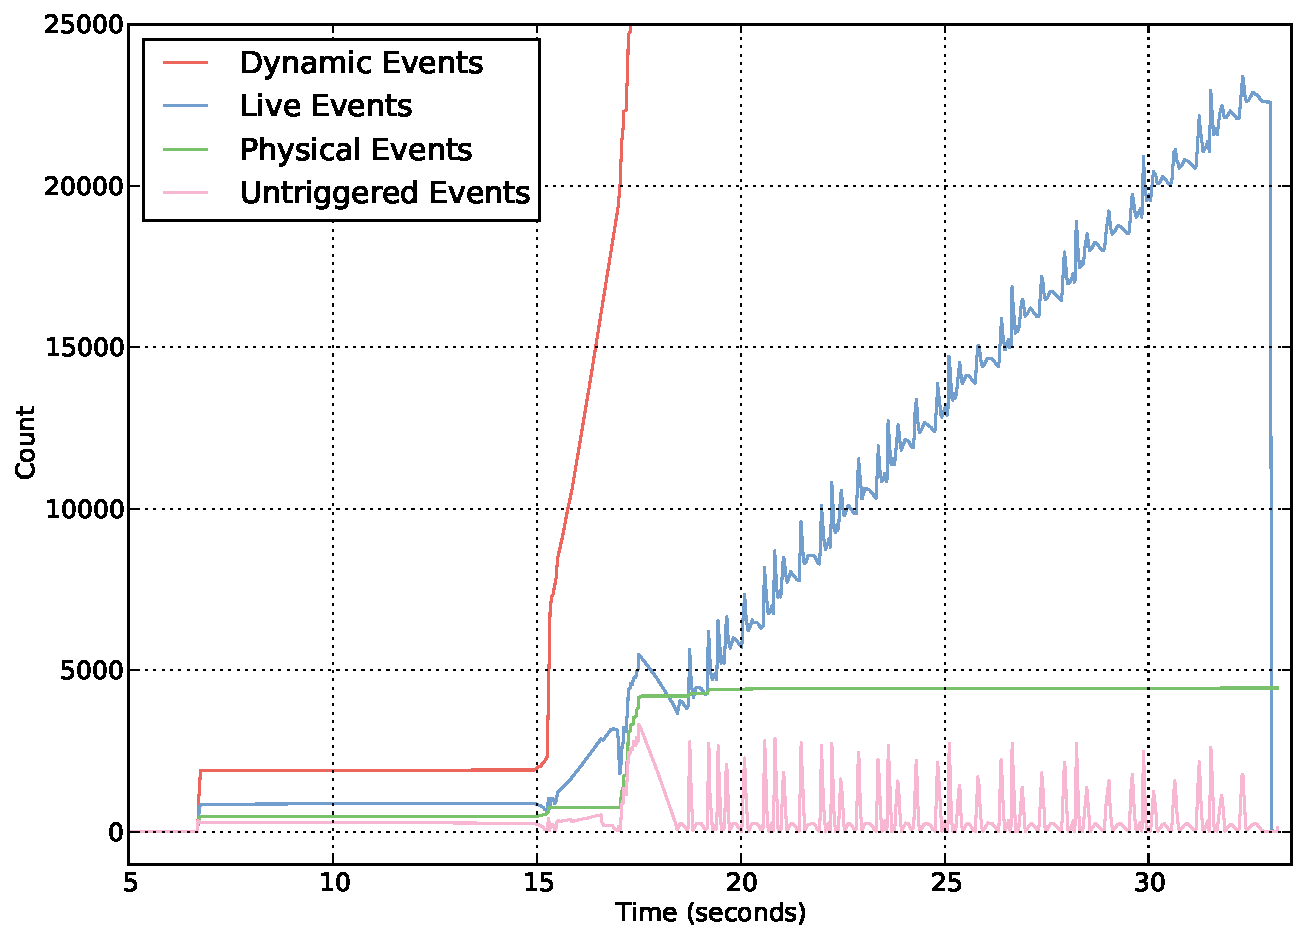
\includegraphics[scale=0.33]{figs/event_lifetimes.pdf}
\end{center}
\vspace{-6mm}
\caption{Event Lifetimes - Fluid Application.\label{fig:eventlife}}
\vspace{-4mm}
\end{figure}

%Figure~\ref{fig:eventlife} shows the event lifetimes in a run of the fluid application.  The total number
%of events created during the application is over 260,000.

\subsection{Deferred Lock Migration}
\label{subsec:lockmig}

We also instrumented our heterogeneous implementation to profile the usage of 
deferred locks in real applications.  We measured how many locks were used in the application.  For
each lock we measured the number of lock requests and the number of times that the lock
had to be transferred from one node to another.  Figure~\ref{fig:lockcount} shows the results 
for the Circuit and AMR application, both running on 16 nodes.  The Circuit application uses
a larger number of locks (3336 vs. 1393), but most of them (86\%) are only used on the node on 
which they were created.  The AMR application exhibits more varied locking behavior, and in 
particular has locks that are requested more often than they are transferred.  In addition
to allowing synchronization in an asynchronous environment, deferred locks must be able to 
migrate to implement real applications on distributed machines.

%Without the
%ability for locks to migrate, these applications couldn't have made use of asynchronous
%locks.

\begin{figure}
\centering

\subfigure[Circuit application]{
\label{fig:lockcount:ckt}
{
\renewcommand{\arraystretch}{1.2}
\small
\begin{tabular}{c|rrrrrrr}
\multicolumn{1}{l}{\multirow{2}{*}{{\renewcommand{\arraystretch}{1}\begin{tabular}{@{}l}\bf Lock\\\bf Xfers\end{tabular}}}}
& \multicolumn{7}{c}{\bf Total Lock Requests} \\
     & 
\multicolumn{1}{c}{\bf 0} &
\multicolumn{1}{c}{\bf 1} &
\multicolumn{1}{c}{\bf 2-8} &
\multicolumn{1}{c}{\bf 9-16} &
\multicolumn{1}{c}{\bf 17-32} &
\multicolumn{1}{c}{\bf 33-64} &
\multicolumn{1}{c}{\bf 65-128} \\
{\bf 0    } & 45 & 2611 & 9   & 26   & 79    & 78    & 30     \\
{\bf 1    } &  -  & 450  &  -   &   -   &   -    &    -   &  -      \\
{\bf 2-8  } &  - & - & - & - & - & - & -\\
{\bf 9-16 } &  -  &  -    &   -  & 8 & - & - & -\\
\end{tabular}
}}
\vspace{-2mm}
\subfigure[AMR application]{
{
\renewcommand{\arraystretch}{1.2}
\small
\begin{tabular}{c|rrrrrrr}
\multicolumn{1}{l}{\multirow{2}{*}{{\renewcommand{\arraystretch}{1}\begin{tabular}{@{}l}\bf Lock\\\bf Xfers\end{tabular}}}}
& \multicolumn{7}{c}{\bf Total Lock Requests} \\
     & 
\multicolumn{1}{c}{\bf 0} &
\multicolumn{1}{c}{\bf 1} &
\multicolumn{1}{c}{\bf 2} &
\multicolumn{1}{c}{\bf 3-4} &
\multicolumn{1}{c}{\bf 5-8} &
\multicolumn{1}{c}{\bf 9-16} &
\multicolumn{1}{c}{\bf 17-32} \\
{\bf 0   } & - & 94  & 592 & 414 & 94 & 3 & 41 \\
{\bf 1   } & - & 122 & -   & -   & -  & - & - \\
{\bf 2   } & - & -   & 6   & 7   & -  & - & - \\
{\bf 3-4 } & - & -   & -   & -   & 9  & 3 & - \\
{\bf 5-8 } & - & -   & -   & -   & -  & - & - \\
{\bf 9-16} & - & -   & -   & -   & -  & 7 & 1
\end{tabular}
}}
\vspace{-2mm}
\caption{Locks by Request and Transfer Counts.\label{fig:lockcount}}
\vspace{-4mm}
\end{figure}

%\subsection{Reduction Case Study}
%\label{subsec:reduccase}

%In this section we give a brief case study of how reductions make it possible
%to achieve high performance on a real application.  One of the three phases
%of the Circuit application involves reducing the current flowing in the wires

\subsection{Bulk-Synchronous Comparison}
\label{subsec:bulkcomp}

Our last set of experiments demonstrates that the asynchronous nature of our interface
is essential to the high performance of the Legion runtime system.  The Legion
implementations of the three applications have already been shown to outperform 
pre-existing implementations\cite{Legion12}.  To quantify the benefit of the asynchronous
nature of our interface, we re-implemented the applications in
a bulk-synchronous style to compare against the existing Legion implementations.  
These bulk-synchronous versions still run on top of 
the Legion runtime, but invoke blocking operations between computational phases,
communication phases, and synchronization.

Figure~\ref{fig:bulksync} compares
the performance of the bulk-synchronous implementations versus the original
implementations for Circuit, Fluid, and AMR.  Each plot contains
performance curves for both implementations on two different problem sizes.
Circuit is a compute-bound application and the bulk-synchronous implementation
performs reasonably well.  By 16 nodes however the overhead grows to 19\%
and 22\% on the small and large inputs respectively.  The Fluid application 
has a more evenly balanced computation-to-communication ratio.  As a result,
Fluid performance suffers significantly more by switching to
a bulk-synchronous model.  At 16 nodes, performance is 135\% and 52\% worse
than the original Legion implementations on the small and large problem sizes
respectively.  Finally, the AMR application is a memory bound application, and on 16 nodes
the bulk-synchronous version is 82\% and 102\% slower on the small and
large problem sizes.

These results show that the asynchronous nature of our interface allows
the Legion runtime system to run ahead of actual execution which
provides significant latency hiding capability.  
The benefit of this latency hiding grows as the number of
nodes increases. % and as the computation-to-communication ratio decreases.
In all cases, the overhead of the bulk-synchronous
implementations grew with the node count.  As we continue to scale
applications to larger and larger machines, the ability of runtimes like Legion to run ahead
will be essential to hiding the large latencies inherent in such machine architectures.
The fully asynchronous nature of the interface presented in this paper
will be crucial for supporting this ability.


\begin{figure}[!ht]
\centering
\subfigure[Circuit Application]{
\label{fig:cktbulk}
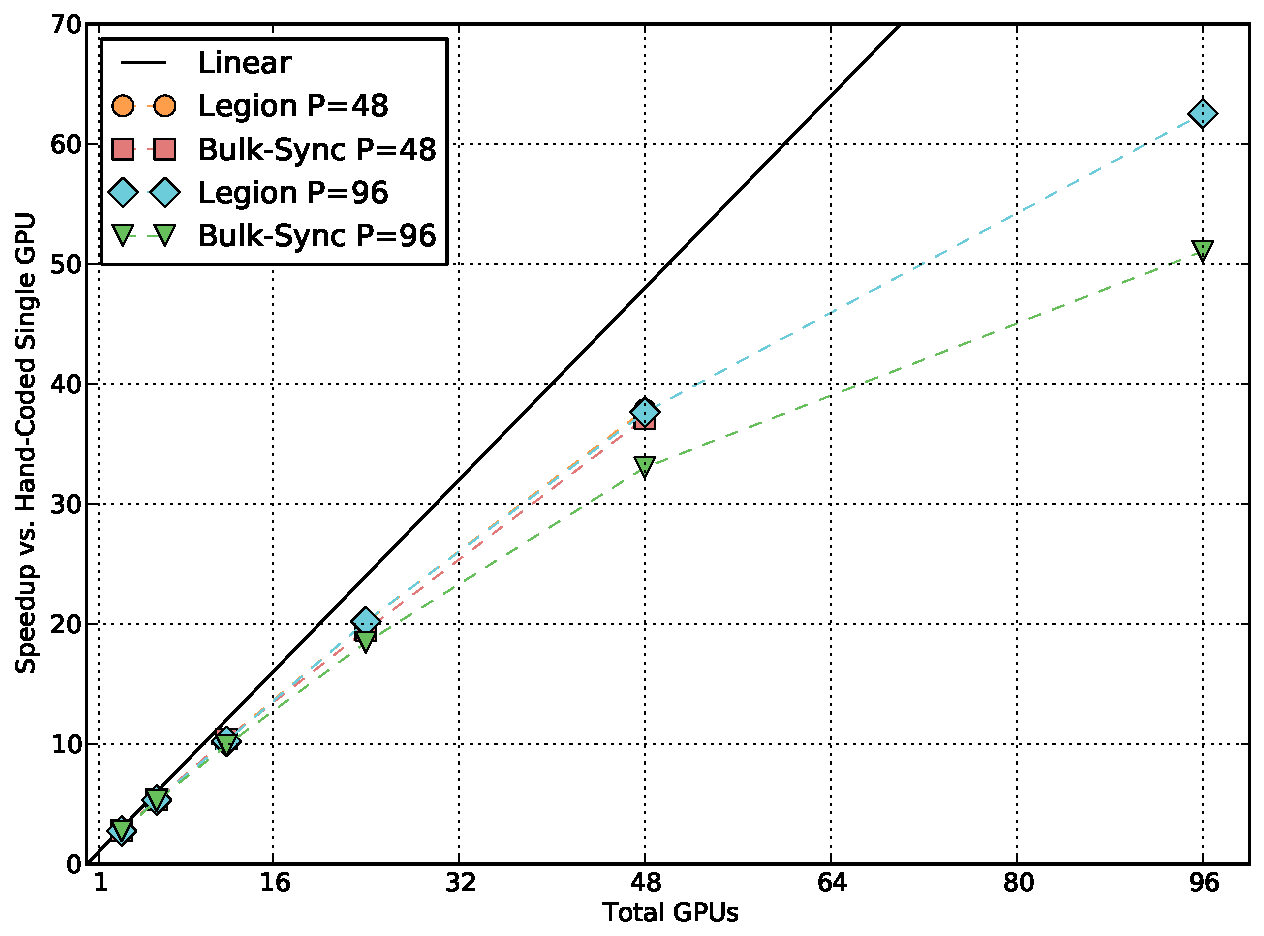
\includegraphics[scale=0.33]{figs/circuit_bulk_sync.pdf}
}

\subfigure[Fluid Application]{
\label{fig:fluidbulk}
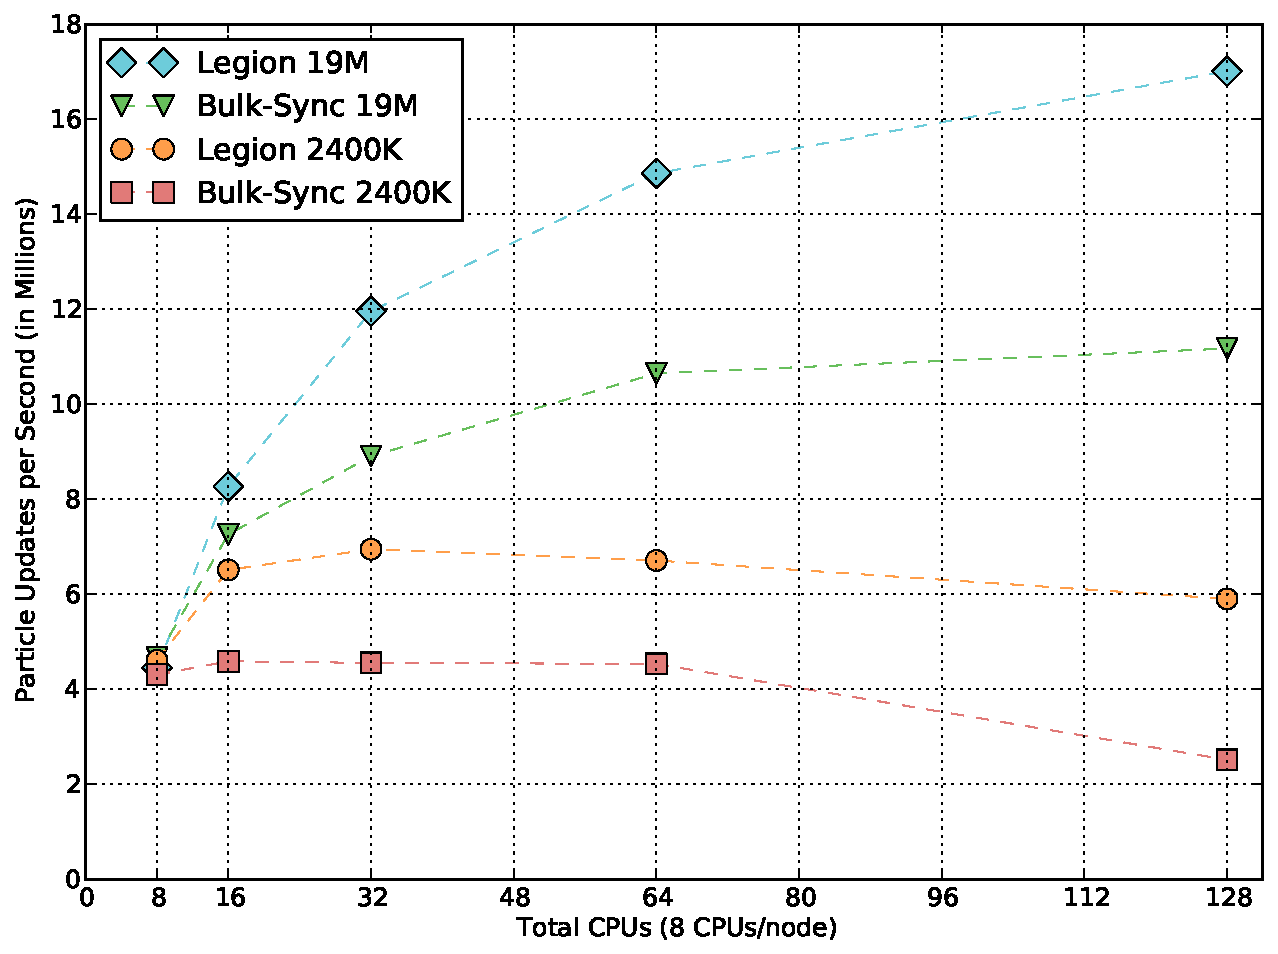
\includegraphics[scale=0.33]{figs/fluid_bulk_sync.pdf}
}

\subfigure[AMR Application]{
\label{fig:amrbulk}
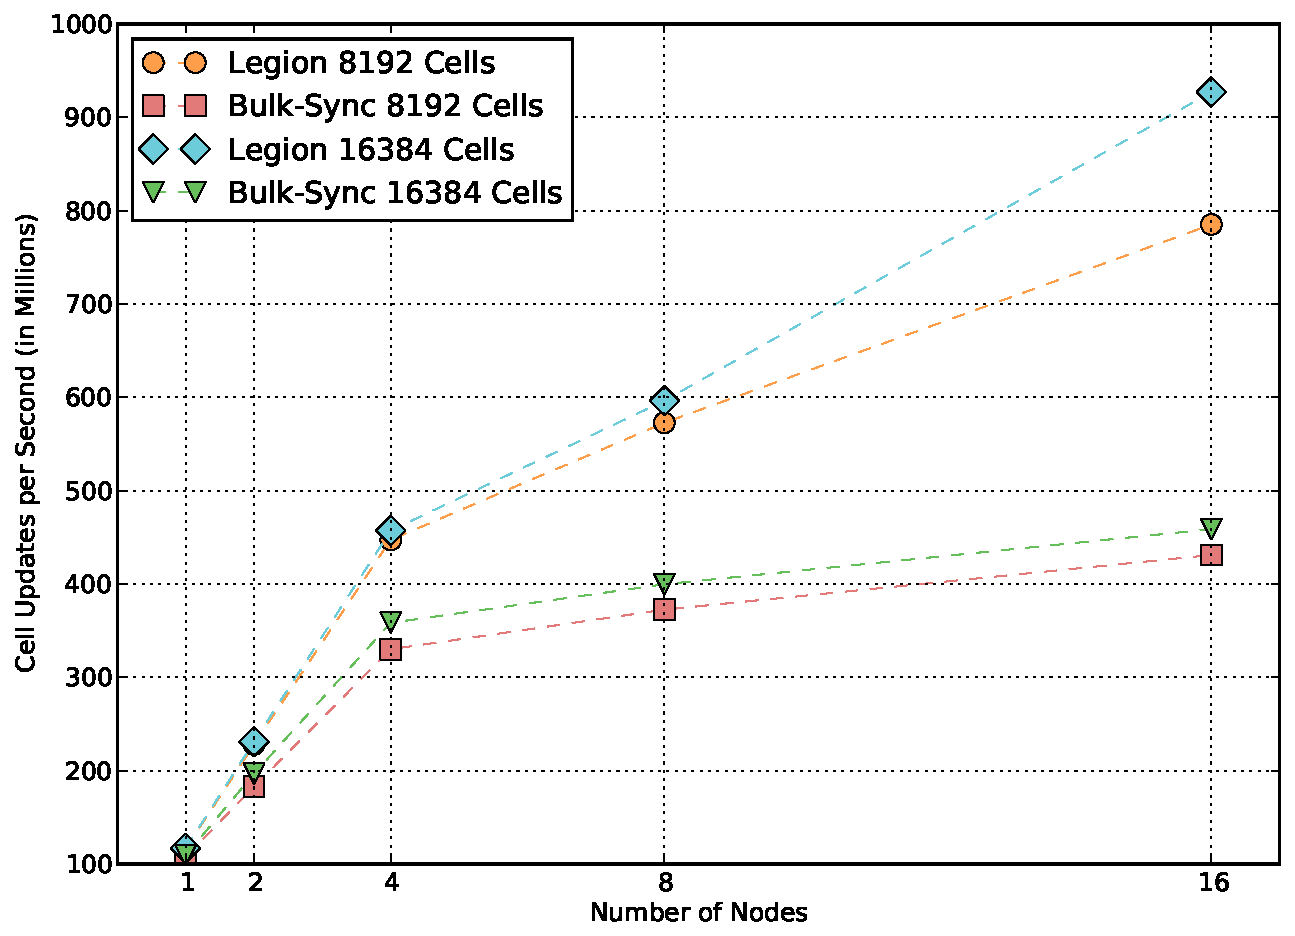
\includegraphics[scale=0.33]{figs/amr_bulk_sync.pdf}
}
\vspace{-4mm}
\caption{Bulk-Synchronous Performance.\label{fig:bulksync}}
\vspace{-4mm}
\end{figure}


